
% some equations

%$\bm{v} ^ \top \bm{A} = \lambda \bm{v} ^ \top$
%$s \bm{v}$
%$s \in \mathbb{R}, s \neq 0$
%$\bm{v} ^ {(1)} , \ldots , \bm{v} ^ {(n)}$
%$\lambda _ {1} , \ldots , \lambda _ {n}$
%$\bm{V} = [ \bm{v} ^ {(1)} , \ldots , \bm{v} ^ {(n)} ]$
%${\bm{\lambda} = [ \lambda _ {1} , \ldots , \lambda _ {n} ]} ^ \top$
%$\bm{u} \in {\mathbb{R}} ^ 2$
%$f(\bm{x}) = \bm{x} ^ \top \bm{A} \bm{x}$
%${\| \bm{x} \|} _ 2 = 1$
%$\forall \bm{x}, \bm{x} ^ \top \bm{A} \bm{x} \geq 0$
%$\bm{x} ^ \top \bm{A} \bm{x} = 0 \Rightarrow \bm{x} = 0$

% eq 2.39
%\begin{equation} \tag{2.39}
%  \label{eq_2_39}
%  \bm{A} \bm{v} = \lambda \bm{v}
%\end{equation}

% eq 2.40
%\begin{equation} \tag{2.40}
%  \label{eq_2_40}
%  \bm{A} = \bm{V} diag(\bm{\lambda}) \bm{V} ^ {-1}
%\end{equation}

% eq 2.41
%\begin{equation} \tag{2.41}
%  \label{eq_2_41}
%  \bm{A} = \bm{Q} \bm{\Lambda} \bm{Q} ^ \top
%\end{equation}

% fig 2.3
%\setcounter{figure}{2.3}
%\begin{figure}[h]
%  \begin{center}
%    Effect of eigenvectors and eigen values\par
%    \begin{tikzpicture}[
%        scale=1,
%      ]
%      \begin{axis}[
%        name = plot1,
%        width=6.2cm,
%        height=6.2cm,
%        trim left,
%        xmin = -3,
%        xmax = 3,
%        ymin = -3,
%        ymax = 3,
%        xlabel = $x_0$,
%        xtick = {-3, -2, -1, 0, 1, 2, 3},
%        ylabel = $x_1$,
%        ylabel style = {yshift=-1.5em},
%        ytick = {-3, -2, -1, 0, 1, 2, 3},
%        title = {Before multiplication},
%      ]
%        \draw [blue] \pgfextra{
%          \pgfpathellipse{
%            \pgfplotspointaxisxy{0}{0}
%          }
%          {\pgfplotspointaxisdirectionxy{cos(45)}{sin(45)}}
%          {\pgfplotspointaxisdirectionxy{cos(315)}{sin(315)}}
%        };
%        \draw [->, red] (axis cs:0,0) node {} -- (axis cs:{cos(45)},{sin(45)}) node[right] {$v ^ {(1)}$};
%        \draw [->, red] (axis cs:0,0) node {} -- (axis cs:{cos(315)},{sin(315)}) node[right] {$v ^ {(2)}$};
%      \end{axis}
%
%
%      \begin{axis}[
%        name = plot2,
%        at = (plot1.right of south east),
%        anchor = left of south west,
%        width=6.2cm,
%        height=6.2cm,
%        trim left,
%        xmin = -3,
%        xmax = 3,
%        ymin = -3,
%        ymax = 3,
%        xlabel = $x_0'$,
%        xtick = {-3, -2, -1, 0, 1, 2, 3},
%        ylabel = $x_1'$,
%        ylabel style = {yshift=-1em},
%        ytick = {-3, -2, -1, 0, 1, 2, 3},
%        title = {After multiplication},
%      ]
%        \draw [blue] \pgfextra{
%          \pgfpathellipse{
%              \pgfplotspointaxisxy{0}{0}
%          }
%          {\pgfplotspointaxisdirectionxy{3*cos(45)}{3*sin(45)}}
%          {\pgfplotspointaxisdirectionxy{.5*cos(315)}{.5*sin(315)}}
%        };
%        \draw [->, red] (axis cs:0,0) node {} -- (axis cs:{cos(45)},{sin(45)}) node[right] {$v ^ {(1)}$};
%        \draw [->, red] (axis cs:0,0) node {} -- (axis cs:{cos(315)},{sin(315)}) node[right] {$v ^ {(2)}$};
%        \draw [->, red] (axis cs:0,0) node {} -- (axis cs:{3*cos(45)},{3*sin(45)}) node[above] {$\lambda _ 1 v ^ {(1)}$};
%        \draw [->, red] (axis cs:0,0) node {} -- (axis cs:{.5*cos(315)},{.5*sin(315)}) node[left] {$\lambda _ 2 v ^ {(2)}$};
%      \end{axis}
%
%    \end{tikzpicture}
%    \caption{Effect of eigenvectors and eigenvalues. An example of the effect of eigenvectors and eigenvalues. Here, we have a matrix $\bm{A}$ with two orthonormal eigenvectors, $\bm{v} ^ {(1)}$ with eigenvalue $\lambda _ 1$ and $\bm{v} ^ {(2)}$ with eigenvalue $\lambda _ 2$. \textit{(Left)} We plot the set of all unit vectors $\bm{u} \in {\mathbb{R}} ^ 2$ as a unit circle. \textit{(Right)} We plot the set of all points $\bm{Au}$. By observing the way that $\bm{A}$ distorts the unit circle, we can see that it scales space in direction $\bm{v} ^ {(i)}$ by $\lambda _ i$}
%    \label{fig:2_3}
%  \end{center}
%\end{figure}

Eigendecomposition is a method that try to decomposit matrix into serval simple parts,
  eigenvectors and eigenvalues.

\begin{itemize}
  \item Eigenvector and Eigenvalue

  % eq 2.39
  \begin{equation} \tag{2.39}
    \label{eq_2_39}
    \bm{Av} = \lambda \bm{v}
  \end{equation}

  Try to find a vector $\bm{v}$ that $\bm{Av}$ is the scale of $\bm{v}$.
    The scaler $\lambda$ is the eigenvalue that corresponding to this eigenvector.
    The eigenvector is still eigenvector after scaling.

  \item Eigendecomposition

  Concatenate all the eigenvectors $\bm{v} ^ {(1)} , \ldots , \bm{v} ^ {(n)}$
    and corresponding eigenvalues $\lambda _ {1} , \ldots , \lambda _ {n}$
    into matrix $\bm{V} = [ \bm{v} ^ {(1)} , \ldots , \bm{v} ^ {(n)} ]$
    and vector ${\bm{\lambda} = [ \lambda _ {1} , \ldots , \lambda _ {n} ]} ^ \top$
    respectively.

  We could say that the matrix $\bm{A}$ could be decomposed into matrix $\bm{V}$ and vector $\bm{\lambda}$ by:

  % eq 2.40
  \begin{equation} \tag{2.40}
    \label{eq_2_40}
    \bm{A} = \bm{V} diag(\bm{\lambda}) \bm{V} ^ {-1}
  \end{equation}

  \newpage

  \item Real Symmetric Matrix Eigendecomposition

  % fig 2.3
  \setcounter{figure}{2}
  \begin{figure}[ht]
    \begin{center}
      Effect of eigenvectors and eigen values\par
      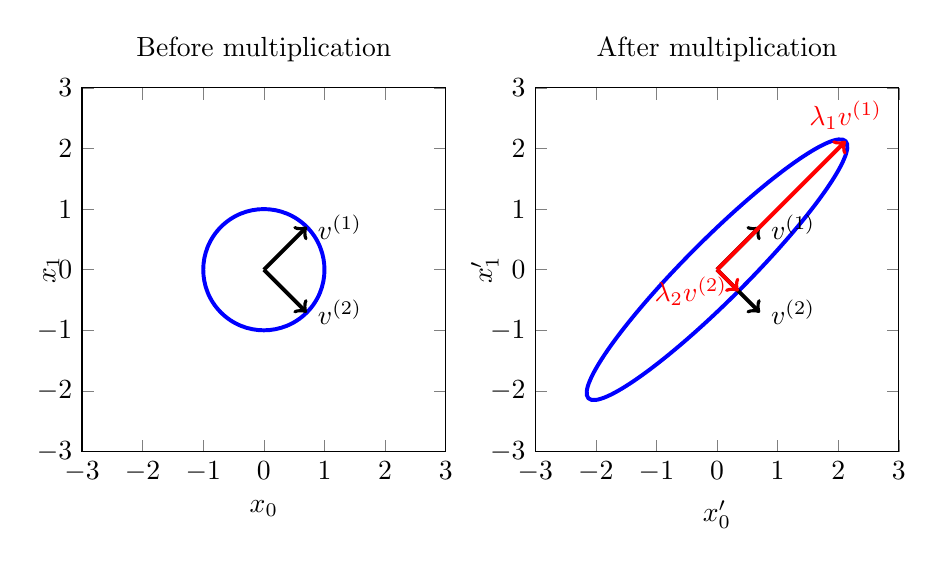
\begin{tikzpicture}[
          scale=1,
        ]
        \begin{axis}[
          name = plot1,
          width=6.2cm,
          height=6.2cm,
          trim left,
          xmin = -3,
          xmax = 3,
          ymin = -3,
          ymax = 3,
          xlabel = $x_0$,
          xtick = {-3, -2, -1, 0, 1, 2, 3},
          ylabel = $x_1$,
          ylabel style = {yshift=-1.5em},
          ytick = {-3, -2, -1, 0, 1, 2, 3},
          title = {Before multiplication},
        ]
          \draw [blue, line width=0.5mm] \pgfextra{
            \pgfpathellipse{
              \pgfplotspointaxisxy{0}{0}
            }
            {\pgfplotspointaxisdirectionxy{cos(45)}{sin(45)}}
            {\pgfplotspointaxisdirectionxy{cos(315)}{sin(315)}}
          };
          \draw [->, line width=0.5mm] (axis cs:0,0) node {} -- (axis cs:{cos(45)},{sin(45)}) node[right] {$v ^ {(1)}$};
          \draw [->, line width=0.5mm] (axis cs:0,0) node {} -- (axis cs:{cos(315)},{sin(315)}) node[right] {$v ^ {(2)}$};
        \end{axis}


        \begin{axis}[
          name = plot2,
          at = (plot1.right of south east),
          anchor = left of south west,
          width=6.2cm,
          height=6.2cm,
          trim left,
          xmin = -3,
          xmax = 3,
          ymin = -3,
          ymax = 3,
          xlabel = $x_0'$,
          xtick = {-3, -2, -1, 0, 1, 2, 3},
          ylabel = $x_1'$,
          ylabel style = {yshift=-1em},
          ytick = {-3, -2, -1, 0, 1, 2, 3},
          title = {After multiplication},
        ]
          \draw [blue, line width=0.5mm] \pgfextra{
            \pgfpathellipse{
                \pgfplotspointaxisxy{0}{0}
            }
            {\pgfplotspointaxisdirectionxy{3*cos(45)}{3*sin(45)}}
            {\pgfplotspointaxisdirectionxy{.5*cos(315)}{.5*sin(315)}}
          };
          \draw [->, line width=0.5mm] (axis cs:0,0) node {} -- (axis cs:{cos(45)},{sin(45)}) node[right] {$v ^ {(1)}$};
          \draw [->, line width=0.5mm] (axis cs:0,0) node {} -- (axis cs:{cos(315)},{sin(315)}) node[right] {$v ^ {(2)}$};
          \draw [->, red, line width=0.5mm] (axis cs:0,0) node {} -- (axis cs:{3*cos(45)},{3*sin(45)}) node[above] {$\lambda _ 1 v ^ {(1)}$};
          \draw [->, red, line width=0.5mm] (axis cs:0,0) node {} -- (axis cs:{.5*cos(315)},{.5*sin(315)}) node[left] {$\lambda _ 2 v ^ {(2)}$};
        \end{axis}

      \end{tikzpicture}
      \caption{Effect of eigenvectors and eigenvalues. An example of the effect of eigenvectors and eigenvalues. Here, we have a matrix $\bm{A}$ with two orthonormal eigenvectors, $\bm{v} ^ {(1)}$ with eigenvalue $\lambda _ 1$ and $\bm{v} ^ {(2)}$ with eigenvalue $\lambda _ 2$. \textit{(Left)} We plot the set of all unit vectors $\bm{u} \in {\mathbb{R}} ^ 2$ as a unit circle. \textit{(Right)} We plot the set of all points $\bm{Au}$. By observing the way that $\bm{A}$ distorts the unit circle, we can see that it scales space in direction $\bm{v} ^ {(i)}$ by $\lambda _ i$}
      \label{fig:effect_of_eigenvectors_and_eigen_values}
    \end{center}
  \end{figure}

  % eq 2.41
  \begin{equation} \tag{2.41}
    \label{eq_2_41}
    \bm{A} = \bm{Q} \bm{\Lambda} \bm{Q} ^ \top
  \end{equation}

  % TODO: Ch 2.7 page 42
  \eqref{eq_2_41} is derided from \eqref{eq_2_40}.
  $\bm{Q}$ is an orthogonal matrix composed of eigenvectors of $\bm{A}$
  , and $\bm{\Lambda}$ is a diagonal matrix which $\Lambda _ {i,i}$ is associated with the eigenvector in column $i$ of $\bm{Q}$.
  Figure~\ref{fig:effect_of_eigenvectors_and_eigen_values} for the example.

  \newpage

  \item Eigendecomposition Characteristics

  \begin{itemize}

    \item Singular

    matrix is singular $\iff \forall \lambda = 0$

    \item Quadratic Expression Optimization

    if ${\| \bm{x} \|} _ 2 = 1,\ f(\bm{x}) = \bm{x} ^ \top \bm{A} \bm{x}$ is optimal.
    $\bm{x}$ is an eigenvector of $\bm{A}$, the $max(f(\bm{x}))$ is maximum eigenvalue, the $min(f(\bm{x}))$ is minimum eigenvalue.

    \item Positive Definite, Positive Semidefinite, Negative Definite, and Negative Semidefinite
    \begin{itemize}
      \item Positive Definite: $\forall \lambda > 0$

        Extra Characteristics: $\bm{x} ^ \top \bm{A} \bm{x} = 0 \Rightarrow \bm{x} = 0$

      \item Positive Semidefinite: $\forall \lambda \geq 0$

        Extra Characteristics: $\forall \bm{x}, \bm{x} ^ \top \bm{A} \bm{x} \geq 0$

      \item Negative Definite: $\forall \lambda < 0$
      \item Negative Semidefinite: $\forall \lambda \leq 0$
    \end{itemize}

  \end{itemize}

\end{itemize}

